\documentclass[12pt]{jarticle}
\usepackage{TUSIreport}
\usepackage{otf}
\usepackage[dvipdfmx]{graphicx}
\usepackage[dvipdfmx]{color}
\usepackage{amsmath}
\usepackage{amssymb}
\usepackage{color}
\usepackage{hhline}
\usepackage{fancybox,ascmac}
\usepackage{multirow}
\usepackage{url}
\usepackage{bm}
\usepackage{listings,jlisting}
%%%%%%%%%%%%%%%%%%
\lstdefinestyle{py}{
    language={Python},
    backgroundcolor={\color[gray]{.85}},
    basicstyle={\small},
    identifierstyle={\small},
    commentstyle={\small\ttfamily \color[rgb]{0,0.5,0}},
    keywordstyle={\small\bfseries \color[rgb]{1,0,0}},
    ndkeywordstyle={\small},
    stringstyle={\small\ttfamily \color[rgb]{0,0,1}},
    frame={tb},
    breaklines=true,
    columns=[l]{fullflexible},
    numbers=left,
    xrightmargin=0zw,
    xleftmargin=3zw,
    numberstyle={\scriptsize},
    stepnumber=1,
    numbersep=1zw,
    morecomment=[l]{//}
}
\begin{document}
%%%%%%%%%%%%%%%%%%%%%%%%%%%%%%%%%%%%%%%%%%%%%%%%%%%%%%%%
% 表紙を出力する場合は,\提出者と\共同実験者をいれる
% \提出者{科目名}{課題名}{提出年}{提出月}{提出日}{学籍番号}{氏名}
% \共同実験者{一人目}{二人目}{..}{..}{..}{..}{..}{八人目}
%%%%%%%%%%%%%%%%%%%%%%%%%%%%%%%%%%%%%%%%%%%%%%%%%%%%%%%
\提出者{情報工学実験3}{課題2 パターン認識}
{2021}{6}{3}{4619055}{辰川力駆}
%%%%%%%%%%%%%%%%%%%%%%%%%%%%%%%%%%%%%%%%%%%%%%%%%%%%%%%%%
\共同実験者{}{}{}{}{}{}{}{}
%%%%%%%%%%%%%%%%%%%%%%%%%%%%%%%%%%%%%%%%%%%%%%%%%%%%%%%%%
% 表紙を出力する場合はコメントアウトしない
%%%%%%%%%%%%%%%%%%%%%%%%%%%%%%%%%%%%%%%%%%%%%%%%%%%%%%%%%
\表紙出力
%%%%%%%%%%%%%%%%%%%%%%%%%%%%%%%%%%%%%%%%%%%%%%%%%%%%%%%
% 以下はレポート本体,reportmain.tex に書いてある.
% \inputを使っているが,直接書いても良い.
%%%%%%%%%%%%%%%%%%%%%%%%%%%%%%%%%%%%%%%%%%%%%%%%%%%%%%%
\section{実験の要旨}
データ分析にとって必要不可欠である前処理を演習や課題を通して理解し、
Pythonを用いて実際に行うことでやり方を身に付ける。

\section{実験の目的}
演習や課題を通して、抽出や集約などの基本的なデータ前処理の仕方を理解する。

\section{実験の原理}
データ分析のためには主に、3つの前処理がある。
\begin{enumerate}
    \item 「指標、表、グラフ作成」のための前処理

          指標の計算、表やグラフに簡単に変換できるようなデータを準備することが目的である。
          必要な列 (Column) を全て持ち、
          扱いやすい単位で集約された行 (Row) が必要な範囲分存在するデータを作成する。
    \item 「教師なし学習」の入力のための前処理

          教師なし機械学習モデルに利用する説明変数を持つデータを準備することが目的である。
          1と同様なデータであるが、
          機械学習モデルの種類に応じて扱いやすいデータの型に変換したり、
          データのスケールを揃えたりする前処理が必要になる。
    \item 「教師あり学習」の入力のための前処理

          教師あり機械学習モデルに利用する学習データ、
          テストデータ、そしてモデルに適用するデータの準備をすることが目的である。
          1や2と同様の前処理だけでなく、例えば、
          複数の列を組み合わせて新たな特徴量に変換する前処理などが必要になることがある。

\end{enumerate}

こういった前処理の目的や役割があるが、
実際に前処理を進めていくにあたっての流れは、
データ構造を対象とした前処理とデータ内容を対象とした前処理に分けている。
\begin{enumerate}
    \item データ構造を対象とした前処理

          複数の行にまたがったデータ全体に及ぶ処理であり、
          前処理の中でも早い段階で実施されることが多い。
          例えば、特定のデータを抽出したり、データを結合したり、
          あるルールに従って複数の行を1行にしたりする。

    \item データ内容を対象とした前処理

          行ごとのデータの値に応じた処理で、
          行ごとに独立で処理できる。
          比較的規模の小さい処理で、
          条件を変えて繰り返されることが多い。
          例えば、
          複数の列を組み合わせて新たな列を生成したり、
          日時のデータを月毎のデータに集約したりする。
\end{enumerate}

\clearpage

\section{実験方法}
PythonをJupyter Notebook上で実行することで、今回の実験を行う。


\subsection{課題1}
reserve\_tbから$50%$の確率で顧客をサンプリングする。
サンプリングした各顧客ごとの予約件数を調査して平均を求める。
顧客のサンプリングに関して以下の2つのやり方で行う。

reserve\_tbの行を$50%$サンプリングした後に顧客を重複なく列にした場合と、
reserve\_tbから重複のない顧客の列を抽出し$50%$
サンプリングをした場合で予約件数の平均がどの様に変わるかを確認し考察する。

\subsection{課題2}
\subsection{課題3}
\subsection{課題4}

\clearpage
\subsection{結果・検討・考察}
実験結果の図2,3より、
myaverage\_integral() は、myaverage\_naive() より処理速度が速い。
これを計算量の観点から考える。

myaverage\_naive() は、画像の高さ(px)$\times$幅(px)$\times$ フィルタサイズ $\times$ フィルタサイズ
であるから、O($n^4$)である。
それに対し、myaverage\_integral() は、画像の高さ(px)$\times$幅(px)のみなので、O($n^2$)である。
これは挿入ソートやバブルソートなどの遅めのソートに匹敵する。

よって、積分画像の平均化フィルタの方が高速化できていることが計算量の観点からも分かる。
図3において、myaverage\_integral()がフィルタサイズの影響をあまり受けてない理由も同様である。




\begin{figure}[h]
    \begin{center}
        %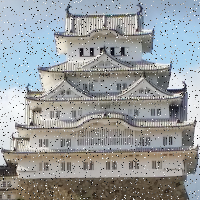
\includegraphics[scale=0.7]{kadai4_2_3.png}
    \end{center}
    \caption{himeji\_noise.png}
\end{figure}

\section{まとめ}
パターン認識とは,入力データを複数のクラスに対応させる処理のことである.

\clearpage
\appendix
\section{付録}

\begin{lstlisting}[style = py,caption=kadai1]
    #4619055
    import time
    import numpy as np
    from skimage.io import imread, imsave
    from skimage.color import rgb2gray, gray2rgb
    from skimage.transform import resize
    from scipy.ndimage.filters import convolve, correlate
    import skimage.transform
    import matplotlib.pyplot as plt
    %matplotlib inline
\end{lstlisting}


%%%%%%%%%%%%%%%%%%%%%%%%%%%%%%%%%%%%%%%%%%%%%%%%%%%%%%%
\end{document}